\appendix
\section{Levels used in Evaluation}
\begin{figure}[H]%
    \begin{center}%
        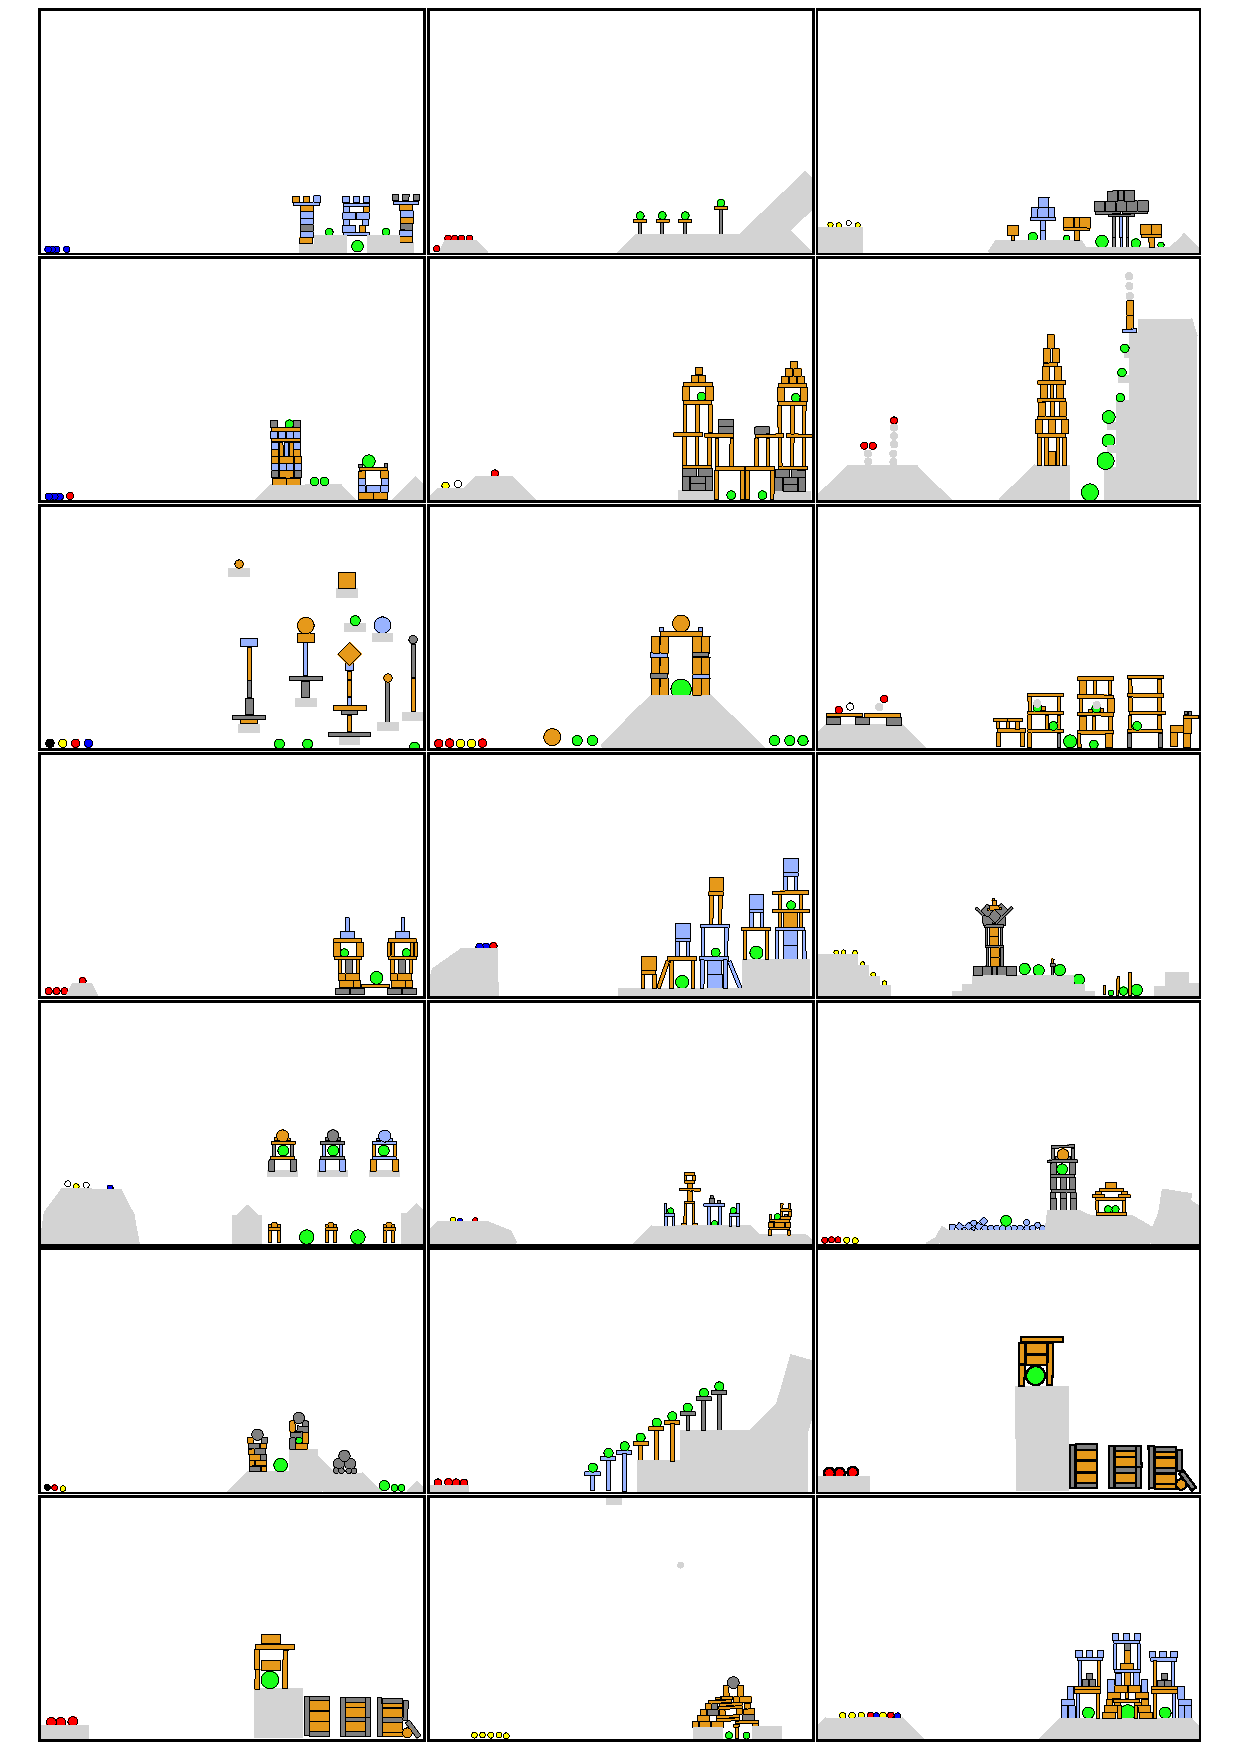
\includegraphics[width=14cm]{data/levels}%
        \vskip -0.3cm%
        \caption{Levels used in Evaluation, 1 through 21, Screenshot from Debugging Tool}%
        \vskip -0,2cm%
        \label{fig:levels}%
    \end{center}%
\end{figure}%
\clearpage
\section{Relations based on Interval Algebra}
\begin{table}[H]
    \centering
    \begin{tabular}{|c|ccc|}
        \hline
        Illustration                                                                                                                 & \multicolumn{1}{l|}{EIA}    & \multicolumn{1}{l|}{IA}                        & \multicolumn{1}{l|}{RIA}       \\ \hline
        \begin{tikzpicture}\draw (-2,0) -- node[above] {a} ++(2,0);\draw (0.5,-0.2) -- node[below] {b} ++(2,0);\end{tikzpicture}     & \multicolumn{3}{c|}{before}                                                                                   \\ \hline
        \begin{tikzpicture}\draw (-2,0) -- node[above] {a} ++(2.5,0);\draw (0.5,-0.2) -- node[below] {b} ++(2.5,0);\end{tikzpicture} & \multicolumn{2}{c|}{meets}  & contact                                                                         \\ \hline
        \begin{tikzpicture}\draw (-2,0) -- node[above] {a} ++(3,0);\draw (-1,-0.2) -- node[below] {b} ++(3,0);\end{tikzpicture}      & \multicolumn{1}{c|}{mom}    & \multicolumn{1}{c|}{\multirow{4}{*}{overlaps}} & \multirow{2}{*}{overlaps most} \\ \cline{1-2}
        \begin{tikzpicture}\draw (-2,0) -- node[above] {a} ++(4,0);\draw (0.5,-0.2) -- node[below] {b} ++(2,0);\end{tikzpicture}     & \multicolumn{1}{c|}{lom}    & \multicolumn{1}{c|}{}                          &                                \\ \cline{1-2} \cline{4-4}
        \begin{tikzpicture}\draw (-2,0) -- node[above] {a} ++(2,0);\draw (-1.2,-0.2) -- node[below] {b} ++(4,0);\end{tikzpicture}    & \multicolumn{1}{c|}{mol}    & \multicolumn{1}{c|}{}                          & \multirow{9}{*}{contact}       \\ \cline{1-2}
        \begin{tikzpicture}\draw (-2,0) -- node[above] {a} ++(2,0);\draw (-0.5,-0.2) -- node[below] {b} ++(2,0);\end{tikzpicture}    & \multicolumn{1}{c|}{lol}    & \multicolumn{1}{c|}{}                          &                                \\ \cline{1-3}
        \begin{tikzpicture}\draw (-2,0) -- node[above] {a} ++(2,0);\draw (-2,-0.2) -- node[below] {b} ++(3,0);\end{tikzpicture}      & \multicolumn{1}{c|}{ms}     & \multicolumn{1}{c|}{\multirow{2}{*}{starts}}   &                                \\ \cline{1-2}
        \begin{tikzpicture}\draw (-2,0) -- node[above] {a} ++(2,0);\draw (-2,-0.2) -- node[below] {b} ++(5,0);\end{tikzpicture}      & \multicolumn{1}{c|}{ls}     & \multicolumn{1}{c|}{}                          &                                \\ \cline{1-3}
        \begin{tikzpicture}\draw (-2,0) -- node[above] {a} ++(2,0);\draw (-2.5,-0.2) -- node[below] {b} ++(6,0);\end{tikzpicture}    & \multicolumn{1}{c|}{ld}     & \multicolumn{1}{c|}{\multirow{3}{*}{during}}   &                                \\ \cline{1-2}
        \begin{tikzpicture}\draw (-2,0) -- node[above] {a} ++(2,0);\draw (-5.5,-0.2) -- node[below] {b} ++(6,0);\end{tikzpicture}    & \multicolumn{1}{c|}{rd}     & \multicolumn{1}{c|}{}                          &                                \\ \cline{1-2}
        \begin{tikzpicture}\draw (-2,0) -- node[above] {a} ++(2,0);\draw (-4,-0.2) -- node[below] {b} ++(6,0);\end{tikzpicture}      & \multicolumn{1}{c|}{cd}     & \multicolumn{1}{c|}{}                          &                                \\ \cline{1-3}
        \begin{tikzpicture}\draw (2,0) -- node[above] {a} ++(4,0);\draw (0,-0.2) -- node[below] {b} ++(6,0);\end{tikzpicture}        & \multicolumn{1}{c|}{mf}     & \multicolumn{1}{c|}{\multirow{2}{*}{finishes}} &                                \\ \cline{1-2}
        \begin{tikzpicture}\draw (4,0) -- node[above] {a} ++(2,0);\draw (0,-0.2) -- node[below] {b} ++(6,0);\end{tikzpicture}        & \multicolumn{1}{c|}{lf}     & \multicolumn{1}{c|}{}                          &                                \\ \hline
        \begin{tikzpicture}\draw (0,0) -- node[above] {a} ++(6,0);\draw (0,-0.2) -- node[below] {b} ++(6,0);\end{tikzpicture}        & \multicolumn{3}{c|}{equal}                                                                                    \\ \hline
    \end{tabular}
    \caption{Illustration of Interval Algebras, without inverse relations}\label{table:relations}
\end{table}